\documentclass[a4paper,10pt,oneside]{article}
\usepackage{graphicx}
\usepackage{color}
\usepackage{url}
\usepackage{subfigure}
\usepackage[utf8]{inputenc}
\usepackage[T1]{fontenc}
\usepackage{tgpagella}
%\usepackage[scale=0.9]{tgcursor}
%\usepackage[scale=0.9]{tgheros}
\usepackage{xstring}

\newcommand{\myscale}{0.74}
\newcommand{\vect}[1]{\boldsymbol{#1}}
\newcommand{\code}[1]{\texttt{\StrSubstitute{#1}{.}{.\.}}}
\def\.{\discretionary{}{}{}}
\newcommand{\jmodule}[1]{\texttt{\textit{#1}}}

\setlength{\hoffset}{-1in} %left margin will be 0, as hoffset is by default 1inch
\setlength{\voffset}{-1in} %analogous voffset
\setlength{\oddsidemargin}{1.5cm}
\setlength{\evensidemargin}{1.5cm}
\setlength{\topmargin}{1.5cm}
\setlength{\textheight}{24cm}
\setlength{\textwidth}{18cm}

\def\mftitle{jInfer AutoEditor Module Description}
\def\mfauthor{Michal Klempa, Mário Mikula, Robert Smetana, Michal Švirec, Matej Vitásek}
\def\mfadvisor{RNDr. Irena Mlýnková, Ph.D., Martin Nečaský, Ph.D.}
\def\mfplacedate{Praha, 2011}
\title{\bf\mftitle}
\author{\mfauthor \\ Advisors: \mfadvisor}
\date{\mfplacedate}

\ifx\pdfoutput\undefined\relax\else\pdfinfo{ /Title (\mftitle) /Author (\mfauthor) /Creator (PDFLaTeX) } \fi

\begin{document}
\maketitle
\noindent Target audience: developers willing to extend jInfer, specifically alter displaying of automata .

\noindent \begin{tabular}{|l|l|} \hline
Responsible developer: & Mário Mikula \\ \hline
Required tokens:       & org.openide.windows.WindowManager \\ \hline
Provided tokens:       & none \\ \hline
Module dependencies:   & Base \\ 
					   & JUNG \\ \hline
Public packages:       & cz.cuni.mff.ksi.jinfer.autoeditor \\ 
					   & cz.cuni.mff.ksi.jinfer.autoeditor.automatonvisualizer \\
   					   & cz.cuni.mff.ksi.jinfer.autoeditor.automatonvisualizer.layouts \\
   					   & cz.cuni.mff.ksi.jinfer.autoeditor.gui.component \\ \hline
\end{tabular}

\section{Introduction}
This is an implementation of a an automaton editor. Using JUNG library, it provides an API to display and modify automata in an interactive mode. For more information on JUNG library, see \cite{jung}.\\

UML diagrams shown in this document are simplified to keep them readable. Simplification involves removing not important class members which are not mentioned in the text, removing members of non-jInfer classes and truncating string of inheritance which are not important for this document.\ For example, \code{VisualizationViewer} class from JUNG library has many methods and does not extends \code{JPanel} class directly, though in an UML diagram it has not any methods and extends \code{JPanel} directly, because it is sufficient for understanding of this document.

\section{Structure}
Structure of \jmodule{AutoEditor} can be divided into following four main parts.
\begin{itemize}
	\item API - API to display automaton in GUI.
	\item Base classes - Classes providing basic functionality that can be extended and combined to achieve desired visualization of an automaton.
	\item Derived classes - Classes derived from the base classes that are used in existing modules and simultaneously serve as examples.
	\item Layout creation - System of creating \code{Layout}s.
\end{itemize}
First, \code{Layout}s and use of base classes to create a visualization of automaton will be described.\\

In case a generic class has a type parameter \code{T}, this has to be the same \code{T} that is used to parametrize jInfer automata. JUNG classes usually need a type parameter for a state and for an edge. These should be then \code{State\textless T\textgreater} (for a state) and \code{Step\textless T\textgreater} (for edge).

\subsection{Layout}
\code{Layout} is a JUNG interface responsible primarily of representation of an automaton and positions of its states. JUNG library provides several implementation of \code{Layout} interface. However, because none of them is convenient for automatic automaton displaying, \jmodule{AutoEditor} provides two additional implementations. \code{Layout} by \emph{Julie Vyhnanovska}, used in her master thesis and \code{Layout} which is using external \emph{Graphviz} software.\\

Class providing creation of \code{Layout} instances is named \code{LayoutHelperFactory}.

\subsubsection{Vyhnanovska Layout} \label{subsubsection:vyhnanovskaLayout}
As mentioned above, this Layout was implemented by \emph{Julie Vyhnanovska} as a part of her master thesis (see \cite{Vyhnanovska}). It positions automaton states on a square grid. This \code{Layout} gives good results for relatively small automata (about 10 states of less) but for larger ones, the results are quite disarranged and confusing.\\

Source code resides in package \code{cz.cuni.mff.ksi.jinfer.autoeditor.automatonvisualizer.layouts.}\\*\code{vyhnanovska}.

\subsubsection{Graphviz Layout} \label{subsubsection:graphvizLayout}
\code{Graphviz Layout} uses \emph{Graphviz}, third-party graph visualization software (see \cite{graphviz}), to create positions of automaton states. To use this \code{Layout}, \emph{Graphviz} has to be installed and path to \emph{dot} binary has to be set in options. This \code{Layout} gives nice results even on large automata.\\

Automaton is transformed to the \emph{dot} representation and the \emph{dot} binary is invoked with this representation on input. It processes the automaton and writes positions of its states to the standard output. The output is then parsed and an instance of \code{Layout} is created using these positions.\\

Source code resides in package\newline \code{cz.cuni.mff.ksi.jinfer.autoeditor.automatonvisualizer.layouts.graphviz}.

\subsubsection{LayoutHelperFactory} \label{subsubsection:LayoutHelperFactory}
In project properties, it is possible to select a \code{Layout} to be used to display automata. \code{LayoutHelperFactory} is a class providing just one static method responsible for creating instances of \code{Layout}s according to a selection in project properties.\\

This method has the following signature.
\begin{verbatim}
public static <T> Layout<State<T>, Step<T>> createUserLayout(
  Automaton<T> automaton,
  Transformer<Step<T>, String> edgeLabelTransformer)
\end{verbatim}
The first argument is an automaton to create layout from. The second is transformer to transform an instance of automaton edge to its string representation, required by the \code{Graphviz Layout}.\\

Source code resides in package \code{cz.cuni.mff.ksi.jinfer.autoeditor.automatonvisualizer.layouts}.

\subsubsection{How to create a new Layout}

New \code{Layout}s can be implemented using the modular system. For information on system of modules, see \cite{archdoc}. To create a new implementation of \code{Layout} interface, it is necessary to create a new class implementing \code{LayoutFactory} interface (package \code{package cz.cuni.mff.ksi.jinfer.autoeditor.automatonvisualizer.layouts}) and annotate it by the following code.

\begin{verbatim}
@ServiceProvider(service = LayoutFactory.class)
\end{verbatim}

Created implementation will be shown in project properties in the \code{Layout} selection.\\

\subsection{Base classes}

\begin{figure}
\centering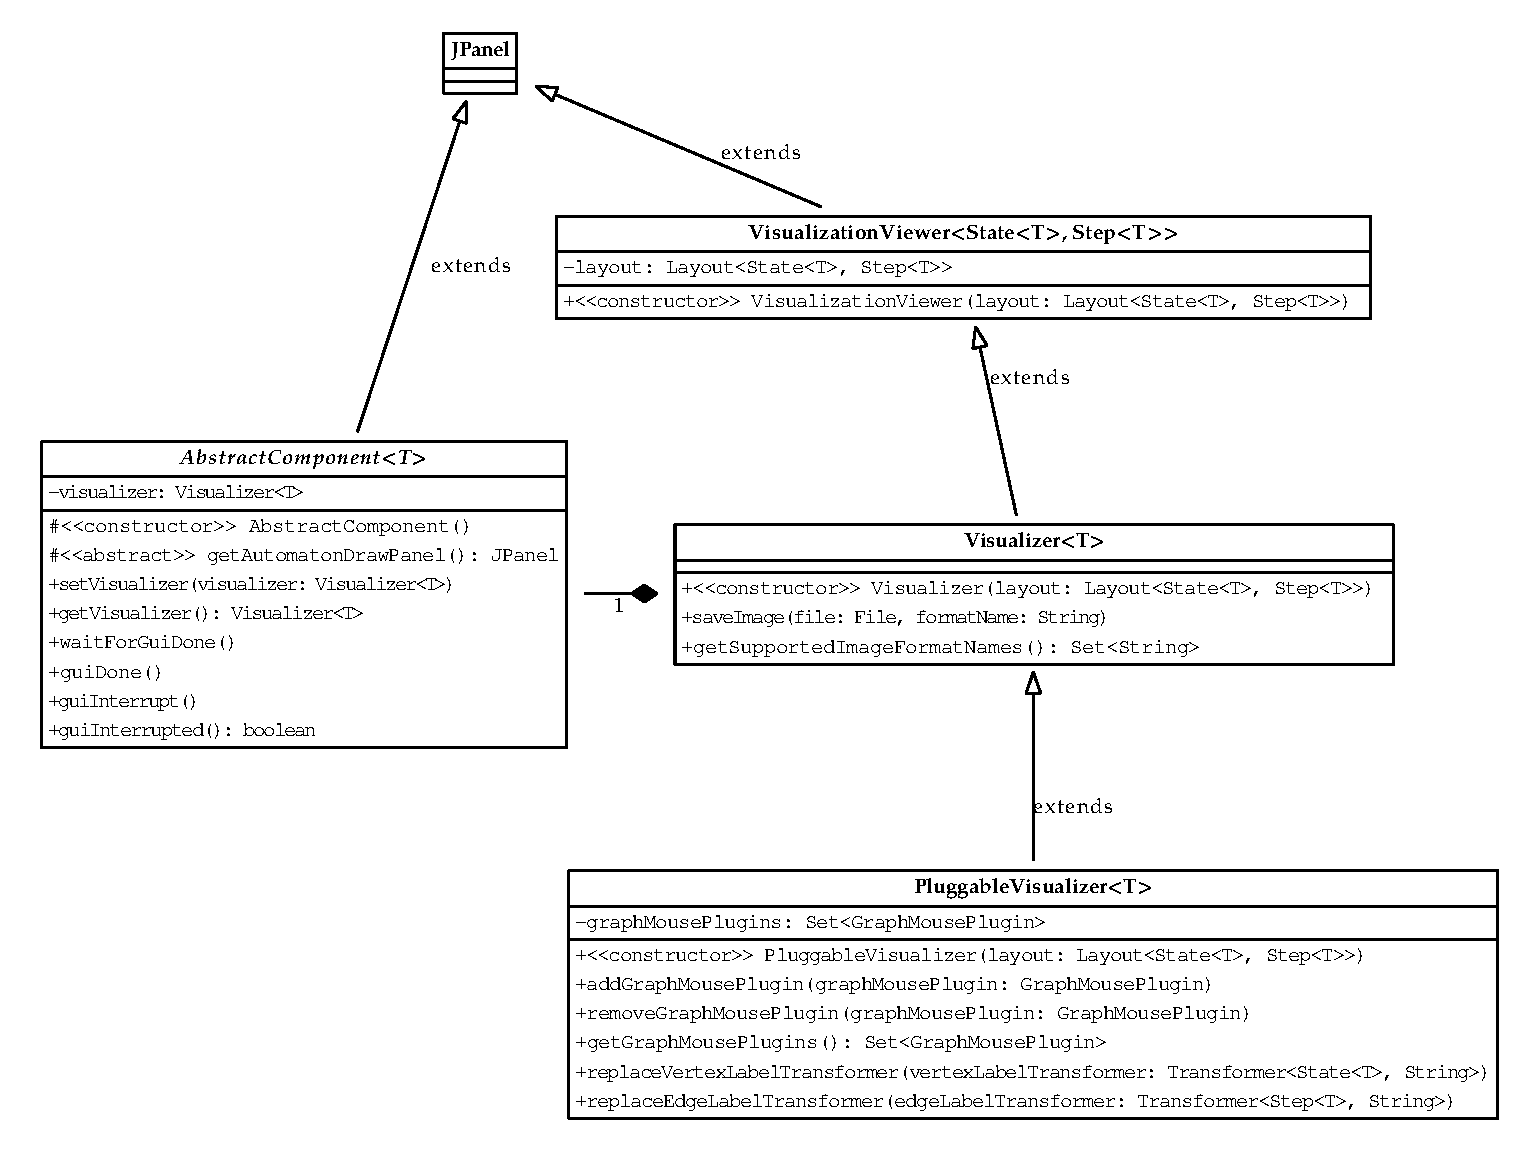
\includegraphics[scale=\myscale]{uml_base_classes}
\caption{Class diagram for the base classes.} \label{uml_base_classes}
\end{figure}

This section describes classes implementing basic common functionality that are supposed to be extended to create a new suitable visualization of automata for a particular method of inference. The new visualization may involve a brand new GUI panel with buttons with various functions, user interaction like selecting states or edges and others.\\

Main two classes representing visualization of automaton are \code{Visualizer} and \code{AbstractComponent}. \code{Visualizer} is a graphical representation of automaton and \code{AbstractComponent} is a panel (extends \code{JPanel}) containing \linebreak the \code{Visualizer} which will be displayed in GUI.\\

\subsubsection{Visualizer}

\code {Visualizer} class in \code{cz.cuni.mff.ksi.jinfer.autoeditor.automatonvisualizer} package extends JUNG \linebreak \code{VisualizationViewer} class thus it inherits all its methods and adds support for saving contained automaton to an image file. Relevant methods are \code{saveImage()} and \code{getSupportedImageFormatNames()}. However, to save an image of automaton it is not necessary to call this methods directly. \jmodule{AutoEditor} GUI contains button to save an image of displayed automaton. For information on how to to this, see \ref{subsection:GUI}.\\

Constructor has one argument, an instance of \code{Layout} interface created from an automaton, typically by \linebreak \code{LayoutHelperFactory} (see \ref{subsubsection:LayoutHelperFactory}).

\subsubsection{PluggableVisualizer}

\code{PluggableVisualizer} class in \code{cz.cuni.mff.ksi.jinfer.autoeditor.automatonvisualizer} package is extension of \code{Visualizer} class, which primarily provides an easy way to plug \emph{graph mouse plugins}.\\

\emph{Graph mouse plugin}s are classes implementing JUNG \code{GraphMousePlugin} interface and their purpose is to enhance \code{Visualizer} with mouse support.\\

By default, instance of \code{PluggableVisualizer} is constructed with two plugins enabled. They are \linebreak \code{ScalingGraphMousePlugin}, providing zooming, and \code{TranslatingGraphMousePlugin}, providing translating the displayed automaton in the x and y direction. In the most cases these plugins are useful, otherwise they can be removed using methods \code{getGraphMousePlugins()} and \code{removeGraphMousePlugin()}.\\

Public (not inherited) methods of \code{PluggableVisualizer} are the following. Their purpose is clear from their names, for details see their JavaDoc.

\begin{itemize}
	\item \code{addGraphMousePlugin()}
	\item \code{removeGraphMousePlugin()}
	\item \code{getGraphMousePlugins()}
	\item \code{replaceVertexLabelTransformer()}
	\item \code{replaceEdgeLabelTransformer()}
\end{itemize}

\subsubsection{AbstractComponent} \label{subsubsection:AbstractComponent}

\code{AbstractComponent} class in \code{cz.cuni.mff.ksi.jinfer.autoeditor.gui.component} package is a representation of GUI panel containing an instance of \code{Visualizer} class for some automaton. It is inherited from \code{JPanel} class, thus provides JPanel's method and behaviour. In addition, it provides the following methods.

\begin{itemize}
	\item \code{setVisualizer()} - Setter of \code{Visualizer}.
	\item \code{getVisualizer()} - Getter of \code{Visualizer}.
	\item \code{waitForGuiDone()} - Suspends its thread until method \code{guiDone} is called on this instance. Do not call this method directly, it is called by \jmodule{AutoEditor}. For more information, see \ref{subsubsection:AbstractComponent user-interactivity support}.
	\item \code{guiDone()} - Wakes up this instance from a suspended state. For detailed description, see \ref{subsubsection:AbstractComponent user-interactivity support}.
	\item \code{guiInterrupt()} - Called when \jmodule{AutoEditor}'s tab is closed to propagate information about terminating of inference to a caller of \jmodule{AutoEditor}. There is no need to called this method directly.
	\item \code{guiInterrupted()} - Checks if \jmodule{AutoEditor} GUI was terminated by \code{guiInterrupt()} method or regularly (\code{guiDone()} method or GUI was not waiting for user interaction). Again, there is no need to call this method directly, it is called by \jmodule{AutoEditor}. For details, see \ref{subsection:GUI}.
\end{itemize}

Besides those methods, \code{AbstractComponent} has one abstract method, named \code{getAutomatonDrawPanel()}.\\

Purpose of this class is to be extended to create own GUI panel, which displays some automaton using a supplied instance of \code{Visualizer}. Method \code{getAutomatonDrawPanel()} is meant to be overridden to return an instance of \code{JPanel}, in which the \code{Visualizer} is to be drawn.\\

Programmer implementing an extension of \code{AbstractComponent} is not forced to place the \code{Visualizer} on his own. It is just needed to create \code{JPanel} and define \code{getAutomatonDrawPanel()} method to return this \code{JPanel}. \jmodule{AutoEditor} will take care of placing and displaying the \code{Visualizer} in the \code{JPanel}.\\

\code{Visualizer} is not set in constructor, because it is often desired to subsequently display several different automata (\code{Visualizer}s) in the same panel. In this case it is not needed to create new instance of \code{AbstractComponent} for each \code{Visualizer}, but subsequently call \code{setVisualizer()} method using one instance of \code{AbstractComponent}.

\subsubsection{AbstractComponent user interactivity support} \label{subsubsection:AbstractComponent user-interactivity support}

If some kind of user interactivity is desired, \code{AbstractComponent} is the right place to implement it.\\

To display the component in GUI and wait for some user action, method \code{waitForGuiDone()} is used. After displaying the component, calling this method suspends the running thread, thus code execution of a caller module is stopped at the place of this call. However, GUI is ran in another thread, user is able to interact with the panel (component).\\*
Do not call method \code{waitForGuiDone()} directly. It is called by \jmodule{AutoEditor} when displaying the component by \jmodule{AutoEditor} \emph{API} method named \code{drawComponentAndWaitForGUI()}. For more information on \jmodule{AutoEditor} \emph{API}, see \ref{subsection:API}.\\

Method important for a programmer extending \code{AbstractComponent} is called \code{guiDone()}. This method wakes up the thread suspended in \code{waitForGuiDone()} method and the programmer is responsible for calling it. Typically, it is called upon some user action like button click, vertex pick or other GUI event.\\*
After calling of \code{guiDone()} method, code execution of the caller module is resumed and holding instance of the \code{AbstractComponent} it is able to retrieve results of user interaction, saved in its state.\\

For examples of user-interactive component, see \ref{subsubsection:StatePickingComponent} and \ref{subsubsection:StatesPickingComponent}. 

\subsection{API} \label{subsection:API}

\jmodule{AutoEditor} \emph{API} is pretty simple. Package \code{cz.cuni.mff.ksi.jinfer.autoeditor} contains class \code{AutoEditor} with three public static methods.

\begin{itemize}
	\item \code{drawComponentAsync()} - Displays given \code{AbstractComponent} asynchronously in a GUI thread and immediately returns. Use this method to just display automaton, without any user interaction and without waiting for any external event. This method does not support it.
	\item \code{drawComponentAndWaitForGUI()} - Displays given \code{AbstractComponent} in a GUI thread, while the caller thread is suspended until  \code{guiDone()} method of \code{AbstractComponent()} is called. This method can wait for GUI events and thus is convenient for user interaction. How to achieve this is described in detail in \ref{subsubsection:AbstractComponent user-interactivity support}.
	\item \code{closeTab()} - Closes \jmodule{AutoEditor}'s GUI tab and interrupts inference, if running.
\end{itemize}

For examples of API usage, see \ref{subsubsection:StatePickingComponent} and \ref{subsubsection:StatesPickingComponent}.

\subsection{Derived classes}

\begin{figure}
\centering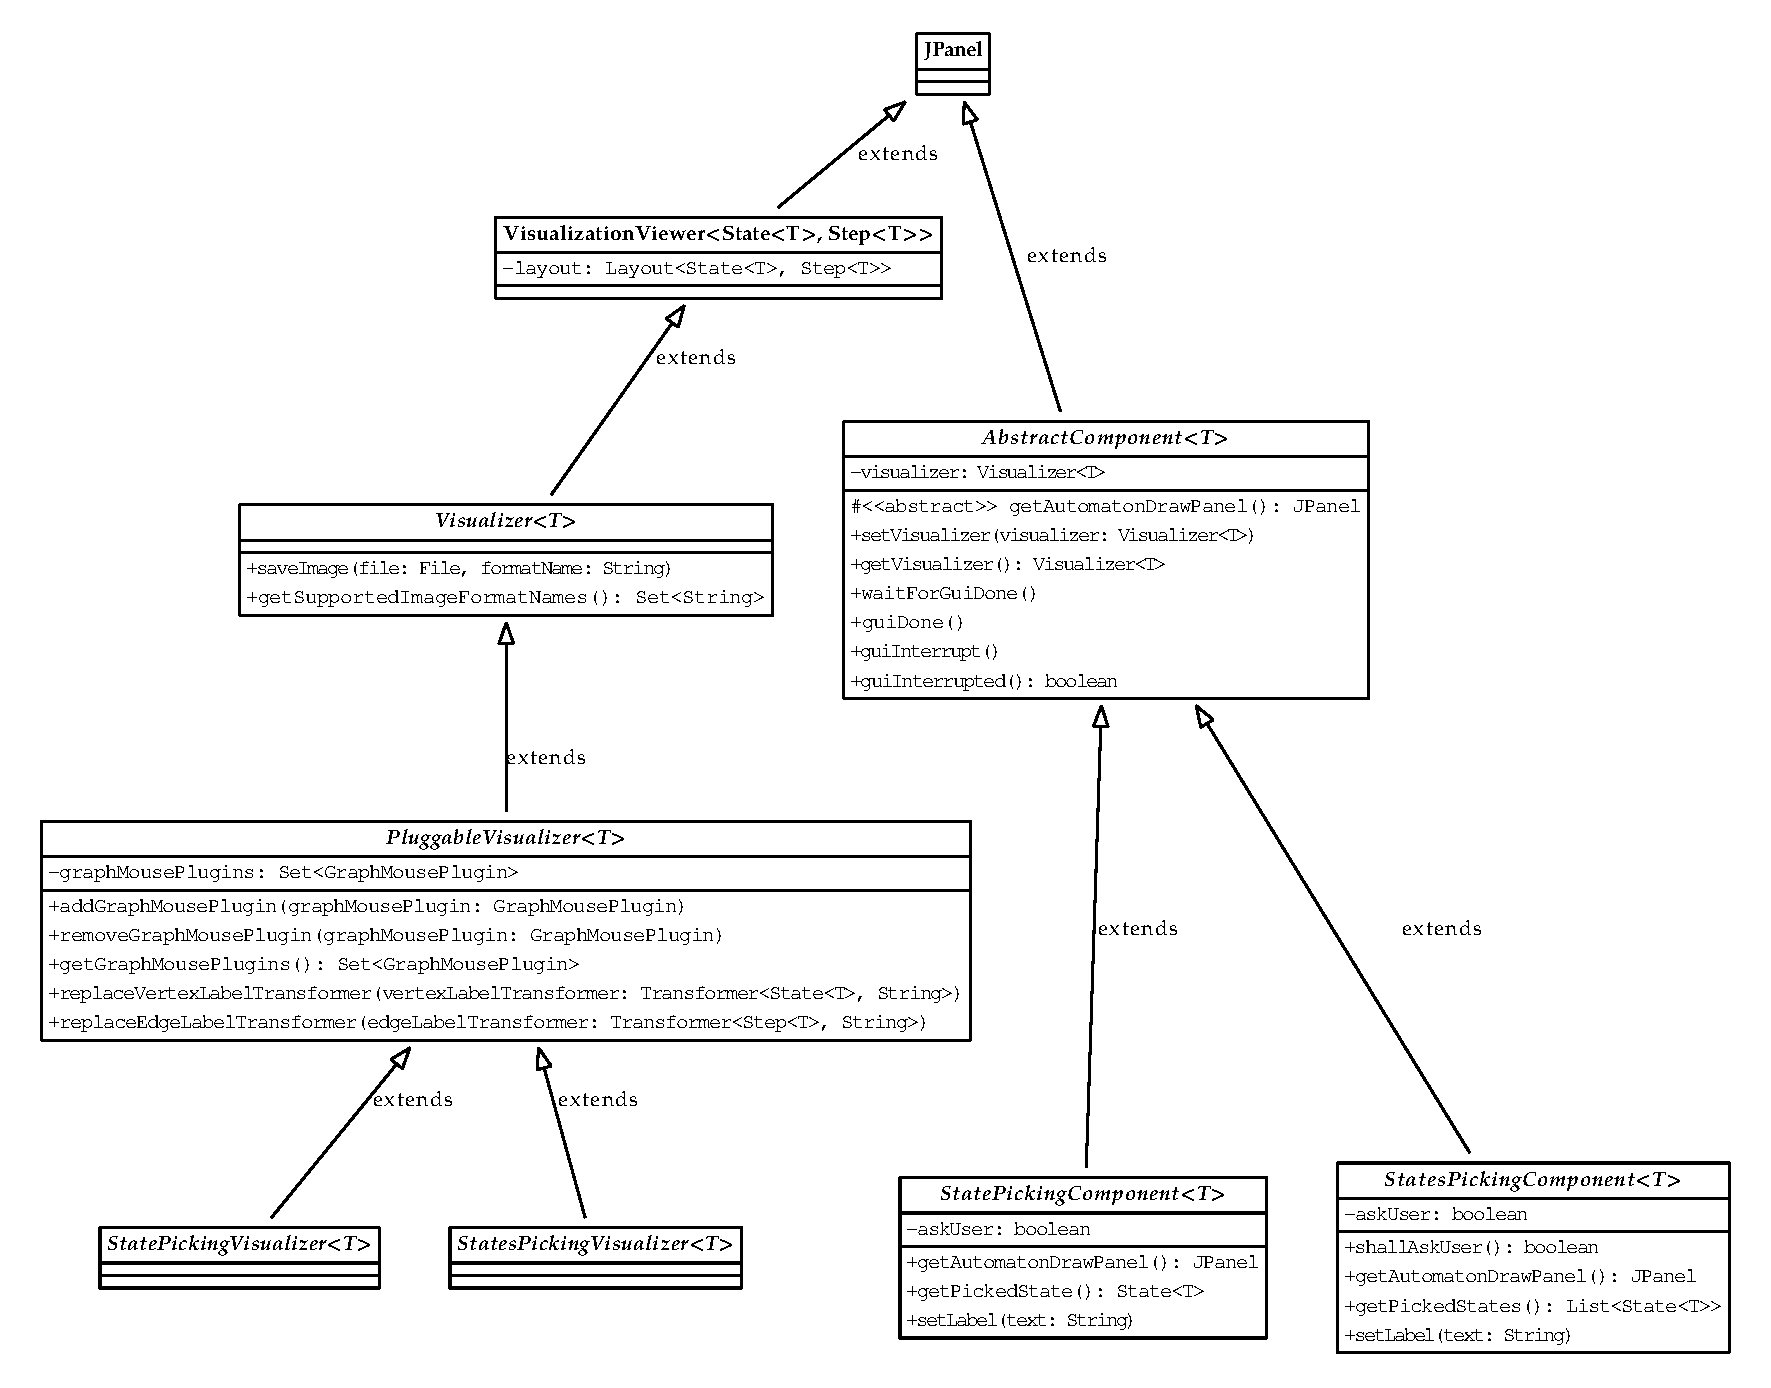
\includegraphics[scale=\myscale]{uml_derived_classes}
\caption{Class diagram for the derived classes, not showing members of classes from figure \ref{uml_base_classes} to keep this diagram simple. Also not showing signatures of constructors of StatePickingVisualizer and StatePickingVisualizer for their length.} \label{uml_derived_classes}
\end{figure}

This section describes classes derived from the base classes used in \jmodule{Two Step Simplifier} module to display automata. This classes may also serve as examples of base classes extensions.

\subsubsection{StatePickingComponent} \label{subsubsection:StatePickingComponent}
\code{StatePickingComponent} (extensions of \code{abstractComponent}) alongside with \code{StatePickingVisualizer} (extension of \code{PluggableVisualizer}) provides possibility to pick one automaton state in GUI and immediately return to the calling code, which can retrieve the picked state.\\

\code{StatePickingVisualizer} is trivial extension of \code{PluggableVisualizer}. It has no additional methods. Its constructor has several additional arguments. Their description follows.
\begin{verbatim}
public StatePickingVisualizer(
    Layout<State<T>, Step<T>> layout,
    Transformer<Step<T>, String> edgeLabelTransformer,
    AbstractComponent<T> component,
    State<T> superinitialState,
    State<T> superfinalState)
\end{verbatim}
\begin{itemize}
	\item \code{layout} - Instance of \code{Layout} which will be provided to the constructor of parent \code{Visualizer} class.
	\item \code{edgeLabelTransformer} - Transformer to convert automaton edges to their string representations.
	\item \code{component} - Instance of \code{AbstractComponent} to call \code{guiDone()} method on, when a state is picked.
	\item \code{superinitialState} and \code{superfinalState} - Superinitial and superfinal states as we want to distinguish these states in displayed automaton.
\end{itemize}

Upon construction, it just adds \code{VertexPickingGraphMousePlugin} to the plugins of \linebreak \code{PluggableVisualizer}. Purpose of this plugin is to allow user to pick some state of automaton and then call \code{guiDone()} method on instance of \code{AbstractComponent}. For description of \code{guiDone()} method, see \ref{subsubsection:AbstractComponent}.\\

\code{StatePickingComponent} provides the following additional methods.
\begin{itemize}
	\item \code{getPickedState()} - After displaying the component using \code{drawComponentAndWaitForGUI()} \emph{API} method (see \ref{subsection:API}), this method retrieves the user picked automaton state.
	\item \code{setLabel()} - Sets text of a component label. The label can be used to communicate some information to user, for example instructions.
\end{itemize}

Source codes of \code{StatePickingComponent} resides in package \code{cz.cuni.mff.ksi.jinfer.autoeditor.gui.}\linebreak\code{component}, \code{StatePickingVisualizer} in \code{cz.cuni.mff.ksi.jinfer.autoeditor.automatonvisualizer} and\linebreak \code{VertexPickingGraphMousePlugin} in \code{cz.cuni.mff.ksi.jinfer.autoeditor.automatonvisualizer.}\linebreak\code{graphmouseplugins}.\\

Example of usage follows.
\begin{verbatim}
    Transformer<Step<Regexp<T>>, String>
      transformer = new Transformer<Step<Regexp<T>>, String>() {
      
        @Override
        public String transform(final Step<Regexp<T>> step) {
          StringBuilder sb = new StringBuilder();
          sb.append("{");
          sb.append(symbolToString.toString(step.getAcceptSymbol()));
          sb.append("|");
          sb.append(String.valueOf(step.getUseCount()));
          sb.append("}");
          return sb.toString();
        }
      };

    State<Regexp<T>> removeState;
    StatePickingComponent<Regexp<T>> component = new StatePickingComponent<Regexp<T>>();
    Layout<State<T>, Step<T>> layout = LayoutHelperFactory.createUserLayout(automaton, transformer);
    StatePickingVisualizer<Regexp<T>>
      visualizer = new StatePickingVisualizer<Regexp<T>>(layout,
                                                         transformer,
                                                         component,
                                                         automaton.getSuperInitialState(),
                                                         automaton.getSuperFinalState());
    component.setVisualizer(visualizer);
    
    do {
      AutoEditor.drawComponentAndWaitForGUI(component);
      removeState = component.getPickedState();

      if ((removeState.equals(automaton.getSuperFinalState()))
           || (removeState.equals(automaton.getSuperInitialState()))) {
        component.setLabel("Do not select superInitial and superFinal states.");
        continue;
      }
      return removeState;
    } while (true);
\end{verbatim}

\subsubsection{StatesPickingComponent} \label{subsubsection:StatesPickingComponent}
\begin{figure}
\centering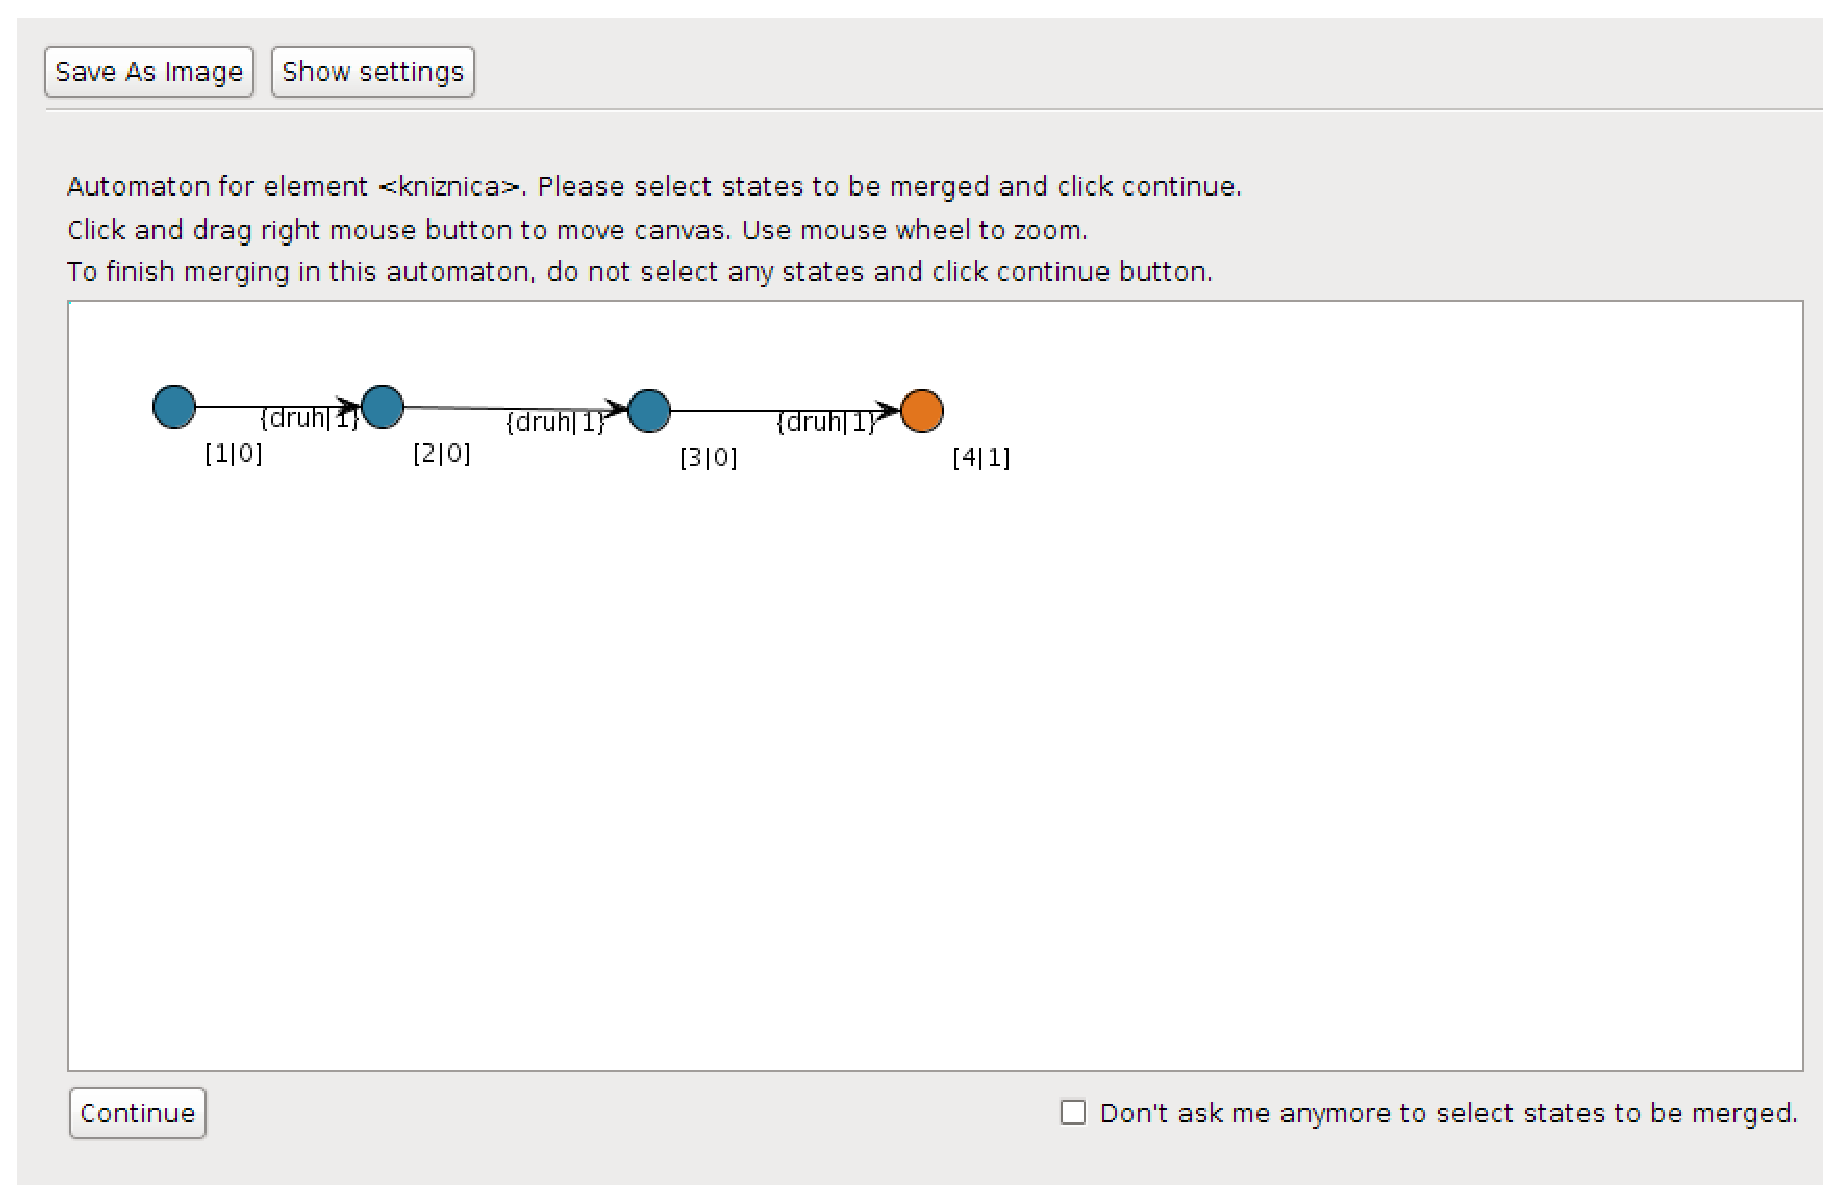
\includegraphics[scale=0.6]{screenshot}
\caption{Screenshot of \jmodule{AutoEditor} GUI} \label{figure_gui}
\end{figure}

Classes \code{StatePickingComponent} and \code{StatesPickingVisualizer} are similar to the classes described in the previous section. Purpose of these is to provide picking of multiple automaton states.\\

\code{StatesPickingVisualizer} is extension of \code{PluggableVisualizer} and upon its construction it adds \linebreak \code{VerticesPickingGraphMousePlugin} to the graph mouse plugins. With this plugin used, user can pick and unpick automaton states separately or pick several states at once by dragging rectangular selection box over states.\
Main difference compared to the \code{VertexPickingGraphMousePlugin} is \code{VerticesPickingGraphMousePlugin} does not call component's \code{guiDone()} method.\\

Signature of constructor and description of arguments follow.
\begin{verbatim}
public StatesPickingVisualizer(Layout<State<T>, Step<T>> layout, Transformer<Step<T>, String> edgeLabelTransformer)
\end{verbatim}
\begin{itemize}
	\item \code{layout} - Instance of \code{Layout} which will be provided to the constructor of parent \code{Visualizer} class.
	\item \code{edgeLabelTransformer} - Transformer to convert automaton edges to their string representations.
\end{itemize}

\code{StatesPickingComponent} is almost the same as \code{StatePickingComponent} but it contains two extra GUI controls. 'Continue' button and 'Don't ask me anymore to select states to be merger' checkbox.\
The button is supposed to be clicked when user picked all desired states and it will cause calling of component's \code{guiDone()} method (see \ref{subsubsection:AbstractComponent}).\
State of the checkbox can be retrieved by the calling code and the caller is supposed to stop showing this component in the current inference process.

Methods of \code{StatesPickingComponent} are the following.
\begin{itemize}
	\item \code{shallAskUser()} - Retrieves state of the checkbox.
	\item \code{getPickedStates()} - After displaying the component using \code{drawComponentAndWaitForGUI()} \emph{API} method (see \ref{subsection:API}), this method retrieves the list of user picked automaton states. In the case that none of automaton states was picked, it returns an empty list.
	\item \code{setLabel()} - Sets text of the component label. The label can be used to communicate some information to user, for example instructions.
\end{itemize}

Source codes of \code{StatesPickingComponent} resides in package \code{cz.cuni.mff.ksi.jinfer.autoeditor.gui.}\linebreak\code{component}, \code{StatesPickingVisualizer} in \code{cz.cuni.mff.ksi.jinfer.autoeditor.automatonvisualizer} and\linebreak \code{VerticesPickingGraphMousePlugin} in \code{cz.cuni.mff.ksi.jinfer.autoeditor.automatonvisualizer.}\linebreak\code{graphmouseplugins}.\\

Example of usage follows.
\begin{verbatim}
  Automaton<T> simplify(Automaton<T> inputAutomaton,
                        SymbolToString<T> symbolToString,
                        String elementName) {
    if (!askUser) {
      return inputAutomaton;
    }

    List<State<T>> mergeLst;
    Transformer<Step<T>, String> transformer = new Transformer<Step<T>, String>() {

      @Override
      public String transform(Step<T> step) {
        StringBuilder sb = new StringBuilder();
        sb.append("{");
        sb.append(symbolToString.toString(step.getAcceptSymbol()));
        sb.append("|");
        sb.append(String.valueOf(step.getUseCount()));
        sb.append("}");
        return sb.toString();
      }
    };

    Boolean selectTwo = false;
    do {
      Layout<State<T>, Step<T>>
        layout = LayoutHelperFactory.createUserLayout(inputAutomaton, transformer);
      StatesPickingVisualizer<T> visualizer = new StatesPickingVisualizer<T>(layout, transformer);

      StatesPickingComponent<T> panel = new StatesPickingComponent<T>();
      panel.setVisualizer(visualizer);
      if (selectTwo) {
        panel.setLabel("Automaton for element <" + elementName
          + ">. Please select states to be merged and click continue. Select at least 2 states.");
      } else {
        panel.setLabel("Automaton for element <" + elementName
          + ">. Please select states to be merged and click continue.");
      }
      
      AutoEditor.drawComponentAndWaitForGUI(panel);
      mergeLst = panel.getPickedStates();

      if ((!BaseUtils.isEmpty(mergeLst)) && (mergeLst.size() >= 2)) {
        inputAutomaton.mergeStates(mergeLst);
        selectTwo = false;
      } else if (mergeLst.size() < 2) {
        selectTwo = true;
      }

      if (!panel.shallAskUser()) {
        askUser = false;
        break;
      }
    } while (!BaseUtils.isEmpty(mergeLst));
    return inputAutomaton;
  }
\end{verbatim}

\subsection{GUI} \label{subsection:GUI}

As shown at figure \ref{figure_gui}, \jmodule{AutoEditor}'s panel is placed in a tab in the editor window. It consists of two buttons, horizontal line below them and a panel to place an extension of \code{AbstractComponent} (see \ref{subsubsection:AbstractComponent}). Class representing this panel is called \code{AutoEditorTopComponent} and resides in \code{cz.cuni.mff.ksi.jinfer.autoeditor.gui.topcomponent} package.\\

Buttons have labels 'Save as Image' and 'Show Settings'. Pushing the first one will raise a dialog box to save currently displayed automaton to an image file. Set of supported image formats depends on installed JRE.\
The second one will open \jmodule{AutoEditor} tab in NetBeans options. For description of the settings, see \ref{subsection:Settings}.

\subsection{Settings} \label{subsection:Settings}

All settings provided by \jmodule{AutoEditor} are NetBeans-wide. The options panel along with all the logic is in the \code{cz.cuni.mff.ksi.jinfer.autoeditor.options} package. Available options include setting the color of the background, colors and shapes of some special types of automaton states.\\

To have some effect, these settings need to be implemented by extensions of \code{Visualizer} class. For examples, see source codes of \code{StatePickingVisualizer} and \code{StatesPickingVisualizer} classes.\\

\nocite{*}
\newpage
\bibliographystyle{alpha}
\bibliography{literature}

\end{document}
